\chapter{线性映射基本定理}

\section{线性映射的秩}
我们已知$\textup{Im }\sigma=\sigma(V_1)=L(\sigma(\alpha_1),\sigma(\alpha_2),\cdots,\sigma(\alpha_n))$,
我们基于此定义线性映射的秩:
\begin{definition}
	设$\sigma\in L(V_1,V_2)$,如果$\sigma(V_1)$是$V_2$的有限维子空间,则
	$\sigma(V_1)$的维数称为$\sigma$的秩,记作$r(\sigma)$,即$r(\sigma)=\dim \sigma(V_1)$.
\end{definition}
简单理解即线性映射的秩即为线性映射像空间的维数.

\section{线性映射基本定理}
这一定理是本学期最重要的定理之一,因其重要性也被冠以线性映射基本定理(有线维线性空间)的名号:
\begin{theorem}
	设$\sigma \in L(V_1,V_2)$,若$\dim V_1=n$,则
	$$r(\sigma)+\dim\ker\sigma=n.$$
\end{theorem}
这一定理的证明方式希望大家熟练掌握,下面是一个思想上类似的例子:
\begin{example}
	设$\sigma$为有限维线性空间$V$上的线性变换,$W$是$V$的子空间,证明:
	$$\dim\sigma(W)+\dim(\sigma^{-1}(0) \cap W)=\dim W.$$
\end{example}
基于线性映射基本定理,我们可以得到如下定理:
\begin{theorem}
	对$\sigma \in L(V_1,V_2)$且$\dim V_1=\dim V_2=n$,我们有
	$\ker\sigma=\{0\}\iff \sigma$为单射$\iff \sigma$为满射$\iff \sigma$为双射(可逆)$\iff r(\sigma)=n$(满秩).
\end{theorem}
显然这一定理前提适用于一切有限维空间上的线性变换.我们需要注意的是,上述第一个等价式不是基于线性映射基本定理得到的,
是教材定理3.1的内容,证明较为容易,建议先自己尝试证明.

线性映射基本定理还隐藏着一个结论,即不可能存在从低维空间到高维空间的满射(反证法代入维数公式即可,当然也可以利用线性相关性证明).

\section{像与核的进一步讨论}
关于线性变换的像和核有很多的包含关系或等式等结论,实际上很多问题都来源于线性映射基本定理及其推论,本节我们主要探讨这一话题.

我们首先说明几个重要的原则:

1. 解决此类问题大多需要综合利用维数公式及其推论,需要讲题给条件转化为合适的等价表述然后解决;

2. 注意集合相等的证明方式,实际上就是两个集合互相包含.实际上很多时候一边的包含是显然的,只需证明另一边;

3. 时刻注意线性映射的像和核的定义,线性空间的交、和与直和的概念,例如看到像需要想到其存在原像,看到和与直和要想到将向量分拆等.

接下来我们看一些经典的结论(已知$V$为有限维线性空间,$\sigma\in L(V,V)$),有余力的同学可以思考其证明,其中结论1最为常见:

1. 若$\sigma$为幂等变换(即$\sigma^2=\sigma$)有$V=\ker\sigma\oplus\textup{Im }\sigma$;

2. $r(\sigma^2)=r(\sigma) \iff V=\ker\sigma\oplus\textup{Im }\sigma$;

3. $\ker\sigma=\ker\sigma^2 \iff \ker\sigma \cap \textup{Im }\sigma=\{0\} \iff \textup{Im }\sigma=\textup{Im }\sigma^2 \iff V=\ker\sigma\oplus \textup{Im }\sigma$;

4. $\ker\sigma \subseteq \ker\sigma^2 \subseteq \ker\sigma^3 \subseteq \cdots$;

5. $\textup{Im }\sigma \supseteq \textup{Im }\sigma^2 \supseteq \textup{Im }\sigma^3 \supseteq \cdots$;

6. 存在正整数$m$使得对任意的$n>m$都有$\ker\sigma^n=\ker\sigma^m$,$\textup{Im }\sigma^n=\textup{Im }\sigma^m$;

7. 存在正整数$m$使得$V=\textup{Im }\sigma^m+\ker\sigma^m$;

8. $\dim(\ker\sigma+\textup{Im }\sigma) \ge \cfrac{n}{2}$,等号成立充要条件为$\ker\sigma=\textup{Im }\sigma$.

\section{可逆与同构}
\subsection{线性空间同构的概念}
\begin{definition}
	如果由线性空间$V_(\mathbf{F})$到$V_2(\mathbf{F})$存在一个线性双射$\sigma$,则称
	$V_(\mathbf{F})$和$V_2(\mathbf{F})$是同构的,记作$V_1(\mathbf{F}) \cong V_2(\mathbf{F})$,
	$\sigma$称为$V_(\mathbf{F})$到$V_2(\mathbf{F})$的一个同构映射.
\end{definition}
容易验证同构为等价关系,且对上述同构映射$\sigma$,$V_1$中向量组$\{\alpha_1,\alpha_2,\cdots,\alpha_m\}$与$V_2$中对应的
$\{\sigma(\alpha_1),\sigma(\alpha_2),\cdots,\sigma(\alpha_m)\}$有相同的线性相关性,这不难证明.

下面是同构的等价条件:
\begin{theorem}
	两个线性空间$V_(\mathbf{F})$和$V_2(\mathbf{F})$同构的充要条件是它们的维数相等.
\end{theorem}
上述即教材定理3.8,定理的证明是简单的,利用维数公式以及同构是等价关系即可.

我们需要指出,同构是本教材中最重要的概念之一,它统一了教材2-3章所学的内容,
将线性空间可以按维数划分为不同的等价类,并且表明线性空间最本质的结构就在于
基及其维数,之前第二章研究的线性相关性与向量组的秩等就是研究线性空间的内部结构,
而线性映射则将相同或不同结构的线性空间联系在一起,同构则表明只要线性空间维数相同,
则可以将两个空间中的所有元素一一对应.
\subsection{线性空间同构举例}
在上一节最后我们提到,同构则表明只要线性空间维数相同,则可以将两个空间中的所有元素
一一对应.本节则研究几个经典的一一对应的例子.

1. 坐标映射:请回顾上一专题中向量的坐标,证明坐标映射是同构映射(实际上是显然的,因为一个
向量在一组基下坐标唯一,而一个坐标对应唯一一个向量);

2. 若$\dim V_1(\mathbf{F})=m$,$\dim V_2(\mathbf{F})=n$,则$L(V_1,V_2) \cong F^{m \times n}$.
证明有两种方式,一种来源于教材定理3.7,较为复杂,我们实际上只需要通过线性映射矩阵表示即可说明.

下面我们通过几个例题进一步了解几个常见的例子(简单题基本只需要判断维数是否相等即可):
\begin{example}
	指出下面各组内的两个线性空间是否同构,若同构可以进一步思考同构映射的构造:

	\textup{(1)}最高次不超过$n-1$的多项式构成的线性空间$\mathbf{R}[x]_n$与$\mathbf{R}^n$;

	\textup{(2)}全体复数在实数域上的线性空间$\mathbf{C}(\mathbf{R})$与$\mathbf{R}^2$;

	\textup{(3)}全体二元复向量$\mathbf{C}^2$在实数域上构成的线性空间$\mathbf{C}^2(\mathbf{R})$与$\mathbf{R}[x]_4$;

	\textup{(4)}全体二元复向量$\mathbf{C}^2$在复数域上构成的线性空间$\mathbf{C}^2(\mathbf{C})$与$L(\mathbf{R}^4,\mathbf{R})$.
\end{example}

\subsection{一些相似的定理}
\begin{theorem}
	\textbf{线性映射对向量坐标的影响}
	
	设$\sigma \in L(V_1,V_2)$关于$V_1$和$V_2$的基$B_1$和基$B_2$的矩阵为$A=(a_{ij})_{m \times n}$,
	且$\alpha$与$\sigma(\alpha)$在基$B_1$和基$B_2$下的坐标分别为$X$和$Y$,则$Y=AX$.
\end{theorem}
上述即教材定理4.1,这一定理给出一个向量经过线性映射之后,其坐标的变化.我们可以用下图表示:
\begin{figure}[h]
	\centering
	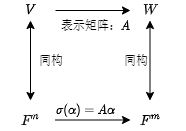
\includegraphics[scale=0.75]{./figs/6/6-1.png}
\end{figure}

图中我们可以看出通过坐标映射后得到的新映射即为定理4.1描述的映射.

在描述下一定理之前,我们首先介绍过渡矩阵(变换矩阵)的概念.
\begin{definition}
	设$B_1=\{\alpha_1,\alpha_2,\cdots,\alpha_n\}$与$B_2=\{\beta_1,\beta_2,\cdots,\beta_n\}$是线性空间
	$V(\mathbf{F})$的任意两组基,$B_2$中每个基向量被基$B_1$表示为
	$$\begin{cases}
		\beta_1=a_{11}\alpha_1+a_{21}\alpha_2+\cdots+a_{n1}\alpha_n \\
		\beta_2=a_{12}\alpha_1+a_{22}\alpha_2+\cdots+a_{n2}\alpha_n \\
		\cdots \\
		\beta_n=a_{1n}\alpha_1+a_{2n}\alpha_2+\cdots+a_{nn}\alpha_n
	\end{cases}.$$
	将上式用矩阵表示为
	$$(\beta_1,\beta_2,\cdots,\beta_n)=(\alpha_1,\alpha_2,\cdots,\alpha_n)\begin{pmatrix}
		a_{11} & a_{12} & \cdots & a_{1n} \\
		a_{21} & a_{22} & \cdots & a_{2n} \\
		\cdots & \cdots &        & \cdots \\
		a_{n1} & a_{n2} & \cdots & a_{nn}
	\end{pmatrix}.$$
	我们将这一矩阵称为即$B_1$变为基$B_2$的变换矩阵(或过渡矩阵).
\end{definition}
简单而言就是将$B_2$中的向量在$B_1$下的坐标按列排列.需要注意表述中是$B_1$变为基$B_2$还是反过来,
这两个矩阵互逆.注意过渡矩阵一定是基与基之间的表示矩阵,并且过渡矩阵一定可逆.
\begin{theorem}
	\textbf{基的选择对向量坐标的影响}
	
	设线性空间$V$的两组基为$B_1$和$B_2$,且基$B_1$到$B_2$的变换矩阵(过渡矩阵)为$A$,如果
	$\xi \in V(F)$,且在$B_1$和$B_2$下的坐标分别为$X$和$Y$,则$Y=A^{-1}X$.
\end{theorem}
上述即教材定理4.10,描述同一个向量在不同基下坐标之间的关系.事实上,这与本节同构关系紧密,因为
同构意味着两个线性空间结构一致,故同构映射可以保持向量组的线性关系不变.在同构关系下,
线性组合对应线性组合,线性无关对应线性无关,线性相关对应线性相关.我们有如下定理:
\begin{theorem}
	设$(\alpha_1,\alpha_2,\cdots,\alpha_n)$是线性无关的向量组,且
	$$(\beta_1,\beta_2,\cdots,\beta_s)=(\alpha_1,\alpha_2,\cdots,\alpha_n)A,$$
	则向量组$(\beta_1,\beta_2,\cdots,\beta_s)$的秩等于矩阵$A$的秩.
\end{theorem}
定理的证明需要用到坐标映射是同构映射这一事实,我们不难发现等式左侧向量组与$A$的列向量组是等价的.
事实上我们也可以由此发现,过渡矩阵一定是可逆矩阵.
\begin{theorem}
	已知$\beta_i=a_{1i}\alpha_1+a_{2i}\alpha_2+\cdots+a_{ni}\alpha_n(i=1,2,\cdots,n)$,
	且$A=(a_{ij})$可逆,则$\alpha_1,\alpha_2,\cdots,\alpha_n$与$\beta_1,\beta_2,\cdots,\beta_n$
	是等价的.
\end{theorem}
实际上这一定理与上一定理的思想都是类似的,我们可以看一个例题练习一下:
\begin{example}
	已知$\beta_1=\alpha_2+\alpha_3$,$\beta_2=\alpha_1+\alpha_3$,$\beta_3=\alpha_1+\alpha_2$,
	证明$\alpha_1,\alpha_2,\alpha_3$与$\beta_1,\beta_2,\beta_3$等价.
\end{example}
\begin{theorem}
	\textbf{基的选择对映射矩阵的影响}
	
	设线性变换$\sigma \in L(V,V)$,$B_1=\{\alpha_1,\dots,\alpha_n\}$和$B_2=\{\beta_1,\dots,\beta_n\}$
	是线性空间的$V(F)$的两组基,基$B_1$变为基$B_2$的变换矩阵为$C$,如果$\sigma$在基$B_1$下的矩阵为$A$,
	则$\sigma$关于基$B_2$所对应的矩阵为$C^{-1}AC$.
\end{theorem}
上述即教材定理7.4,研究同一个映射在不同基下表示矩阵之间的关系.实际上我们将在下一专题初等矩阵一节进一步讨论.
这一定理的证明需要用到我们之前描述的两种线性映射矩阵表示的统一性.

\vspace{2ex} 
\centerline{\heiti \Large 内容总结}

\vspace{2ex} 

\centerline{\heiti \Large 习题}
\vspace{2ex} 
{\kaishu }
\begin{flushright}
    \kaishu

\end{flushright}
\centerline{\heiti A组}
\begin{enumerate}
	\item 
\end{enumerate}
\centerline{\heiti B组}
\begin{enumerate}
	\item 
\end{enumerate}
\centerline{\heiti C组}
\begin{enumerate}
	\item 
\end{enumerate}